\chapter{Test Phase 1}

Comme décrit dans la pré-étude, afin de valider la phase 1 du développement du projet, un test impliquant le capteur choisi ainsi que la passerelle est effectué afin de s'assurer que les deux éléments sont capable de remplir les tâches qui leurs sont attribuées pour le projet. Si le test est concluant alors la solution matérielle choisie peut être validée pour la suite du développement. Dans le cas contraire le matériel doit être changé afin de pouvoir garantir une solution adéquate.

Ce test permet de valider deux éléments, premièrement il vise à vérifier la bon fonctionnement du capteur et de la passerelle dans les conditions finale d'utilisation, c'est à dire une réception adéquate des données envoyées par le capteur en extérieur et en mouvement. De plus ce test va également permettre de choisir la configuration initiale a utiliser pour la transmission des paquets LoRa, en particulier le facteur d'étalement ainsi que la puissance de transmission du signal de sortie à utiliser. On rappelle qu'un petit facteur d'étalement permettra un taux de transfert plus élevé sur une distance moindre, alors qu'un grand facteur permettra l'envoie de données à des distances accrues mais à un taux plus bas. En ce qui concerne la puissance de sortie, l'objectif est de trouver la valeur minimale qui permet une bonne réception des données à la distance prescrite par le cahier des charges, c'est à dire 5 km. Ceci permettra de garantir l'utilisation de la batterie pendant la durée requise de 10h.

Pour pouvoir effectuer ce test les éléments suivants ont été réalisés.

\begin{itemize}
\item Mise en place et assemblage du matériel du capteur et de la passerelle
\item Développement d'un programme de test pour le capteur
\item Installation et configuration du packet forwarder de la passerelle
\item Développement d'une partie du serveur d'application de la passerelle
\end{itemize}

Afin de pouvoir s'assurer de la bonne réception des données le capteur, à intervalles réguliers, va envoyer un paquet de données à destination de la passerelle. Le format ainsi que le contenu du paquet envoyé par le capteur est décrit dans la figure~\ref{fig:test1_paquet}.

\begin{figure}[htb]
\centering 
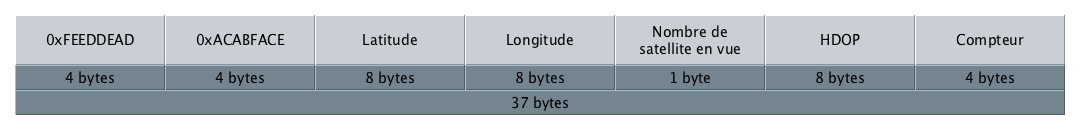
\includegraphics[width=1\columnwidth]{test1_packet_format} 
\caption{Format du paquet test1}
\label{fig:test1_paquet}
\end{figure}

Un programme de test, utilisant le système de développement Arduino IDE proposant un framework pour les cartes Arduino est réalisé. Son comportement est très simple, il se contente d'envoyer un paquet de données LoRa puis d'attendre un certain temps, au terme duquel le cycle recommence. Le paquet envoyé par le capteur commence par deux valeurs fixes suivi de la latitude/longitude du capteur au moment de l'envoie du paquet. Ces deux éléments sont suivis du HDOP, ou Horizontal Dilution of Precision, qui exprime le degré de précision de la position GPS. Pour terminer, la valeur du compteur est ajouté au paquet ce qui permettra à la passerelle de détecter quand un paquet est perdu et ainsi garder des statistiques afin de pouvoir jauger la qualité de la transmission.

Du côté de la passerelle, le packet forwarder, logiciel repris depuis internet, est configuré et mis en œuvre. Il récupère les paquets LoRa reçu et les transmets par le biais d'un paquet UDP. Une partie du serveur d'application est développée qui permet à la passerelle de récupérer les paquets LoRa émit par le packet forwarder et d'en analyser le contenu. A chaque paquet reçu la passerelle s'assure que le paquet est en provenance du capteur en vérifiant la valeur des deux marqueurs de début, ensuite la valeur du compteur est vérifiée pour s'assurer que c'est bien celle attendue, si ce n'est pas le cas cela signifie qu'un ou plusieurs paquets ont été perdus. Cette partie du serveur d'application servira de base pour le développement final de l'application. Au moyen d'un shell implémenté dans le serveur de paquet, il est possible à tout moment de sauver le contenu des paquets reçu jusqu'ici dans un fichier, cela permet ensuite d'en extraire les positions GPS afin de les afficher dans un logiciel comme Google Earth par exemple.

\section{Scénarios}

Deux scénarios distinct sont réalisés en utilisant le système expliqué dans la section précédente. Ils seront effectués deux fois chacun, une fois avec la valeur d'étalement de spectre (spreading factor) avec la plus petite valeur et une fois avec la plus grande valeur, cela permettra de jauger quelle configuration sera nécessaire pour la version finale du capteur.

Le premier test est le test sur piste", il consiste à prendre le capteur et ensuite de marcher le long du parcours d'une piste d'athlétisme. L'objectif de ce test est de voir si dans des conditions proches de l'utilisation finale pour le projet les données sont reçues correctement et de pouvoir également juger de la configuration finale que le système devra utiliser.

Le deuxième test est appellé test de distance, l'objectif et de pouvoir évaluer la distance maximum de fonctionnement jusqu'à laquelle les paquets sont bien reçus. Pour se faire, le capteur sera déplacé sur une ligne droite jusqu'à un point fixé puis il sera ensuite retourné au point de départ.

\subsection{Résultats}

Les résultats des tests décrit dans cette section on été réalisés à la place d'arme de Planeyse à Neuchâtel le 13 Juillet 2018. Cette endroit dispose de grandes surfaces plane et également d'une piste proposant des conditions très proche d'une piste d'athlétisme. C'est donc un endroit idéal réunissant les besoins nécessaire.

\begin{table}[htb]
\caption[Résultats de phase de test 1]{Résultats de phase de test 1}
\label{tab:resultat_test_1}
\centering
\begin{tabular}{ l | l }
\toprule
Test Piste & Planeyse 13.07.2018  \\
\midrule
Microcontrôleur & ATSAMD21G18 – ARM Cortex M0 \\
\bottomrule 
\end{tabular}
\end{table}







